\documentclass{article}
\usepackage{spconf,amsmath,graphicx,booktabs,multirow,amssymb,hyperref,balance}
\hypersetup{hidelinks}

\title{GAZESPOT: HEAD-CONDITIONED SPATIAL GATING AND MULTI-LEVEL FUSION\\
FOR ROBUST GAZE TARGET ESTIMATION}

\name{Bin Fan, Tongjie Pan, Huiyu Zhai, Tao Zhou, Yalan Ye}
\address{School of Computer Science and Engineering,\\
University of Electronic Science and Technology of China, Chengdu, China}

\begin{document}
\ninept
\maketitle

\begin{abstract}
Gaze target estimation with frozen vision foundation models is attractive because it avoids heavy task-specific encoders, yet most existing designs decode only the final feature layer. Such representations can lose the local structure needed to separate nearby people and objects. We present GazeSpot, a single-branch model that combines head-conditioned spatial gating with adaptive multi-level feature fusion. The gate converts relative head coordinates into a soft Spotlight Mask that suppresses unrelated regions, while the fusion module assigns image-dependent weights to features at different backbone depths. The model requires neither depth nor pose inputs and uses no external object detector or segmentation model. Experiments on GazeFollow and VideoAttentionTarget show competitive localization, with consistent gains over a last-layer baseline in crowded scenes. Cross-dataset evaluation on GOO-real further indicates improved robustness without target-domain fine-tuning.
\end{abstract}

\begin{keywords}
gaze target estimation, vision foundation model, spatial gating, multi-level features, crowded scenes
\end{keywords}

\section{Introduction}
Gaze target estimation predicts where a person is looking from an image and a head bounding box~\cite{recasens2015they,chong2020detecting,recasens2017following}. It supports intention understanding, human-computer interaction, and social-scene analysis~\cite{fathi2012learning,zander2010combining,emery2000eyes}. Classical systems encode the cropped head and scene in separate branches~\cite{chong2020detecting,fang2021dual}; later methods incorporate depth, pose, interaction, or object cues~\cite{bao2022escnet,gupta2022modular,tonini2022multimodal,tonini2023object,wang2022gatector}. These designs are effective, but require multiple encoders or additional preprocessing. ViTGaze~\cite{song2024vitgaze} and Gaze-LLE~\cite{ryan2025gaze} simplify the pipeline by coupling a frozen vision foundation model (VFM) with a small gaze decoder.

\begin{figure}[t]
  \centering
  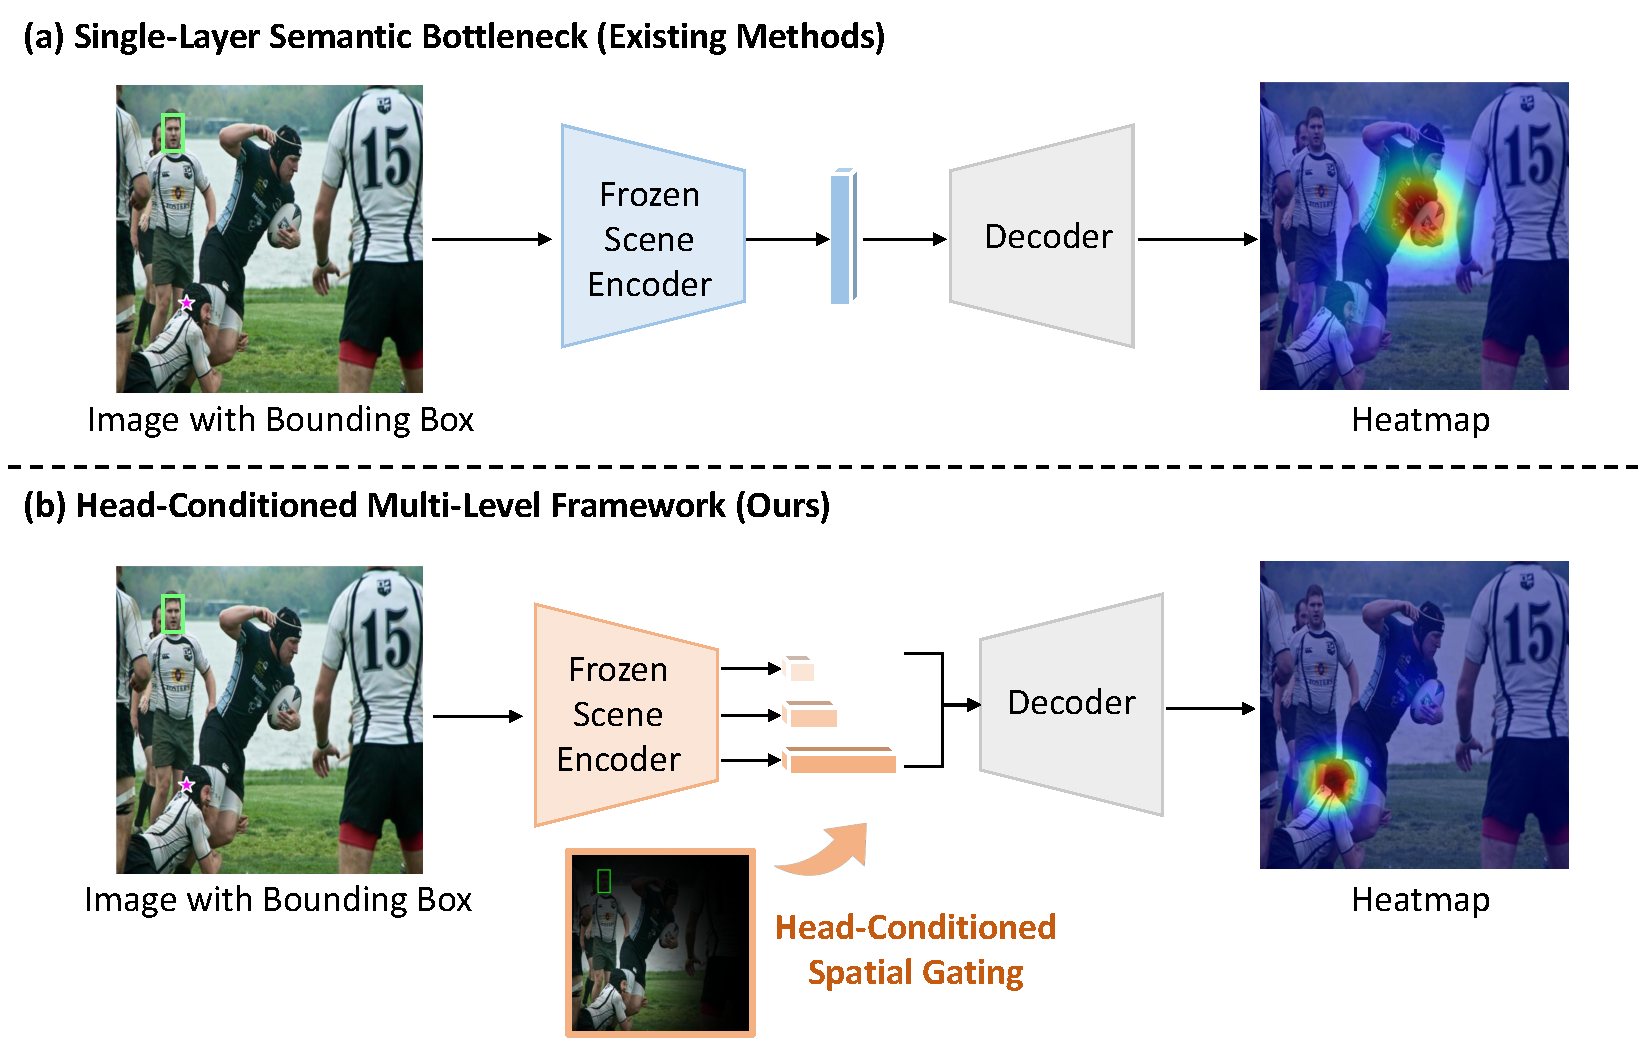
\includegraphics[width=\columnwidth]{img/icasspFig1.pdf}
  \caption{Motivation. Decoding only the final VFM layer can draw the response toward a salient distractor in a crowded scene. GazeSpot instead combines multiple feature levels with a head-conditioned Spotlight Mask, yielding a more concentrated response near the annotated target.}
  \label{fig:motivation}
\end{figure}

The simplicity of a frozen VFM is appealing, but current single-branch models generally decode only its final feature map. Deep features provide strong semantics, whereas point localization also depends on relative position and local boundaries~\cite{kellnhofer2019gaze360}. Hierarchical features are effective in dense prediction~\cite{lin2017feature}, and self-supervised Transformers expose object-localization cues before task-specific training~\cite{caron2021emerging,simeoni2021localizing}. As illustrated in Fig.~\ref{fig:motivation}, this distinction matters when nearby people and objects compete for the decoder's response. Head position is usually added as a mask or embedding at the decoding stage; it does not directly regulate the spatial response of the scene features.

We observe the same issue in the controlled backbone comparison reported in Table~\ref{tab:backbone}(b). With an otherwise unchanged last-layer decoder, replacing DINOv2~\cite{oquab2023dinov2} with DINOv3~\cite{simeoni2025dinov3} increases localization error on GazeFollow and crowded VAT frames. This does not prove feature over-smoothing, but it shows that a stronger final-layer representation does not automatically provide more accurate gaze localization. We therefore retain intermediate features rather than treating the final layer as the only useful representation.

Recent geometric approaches provide another route. Mi et al.~\cite{mi2026objectaware} use DINOv3 features together with object masks from YOLO11x and SAM2, supervise a 2-D gaze direction, and convert it into an angular field-of-view prior. Their object-level formulation is well suited to reasoning over candidate targets. Our aim is different: preserve the compact single-branch setting and require only the head box already assumed by gaze-following benchmarks. We learn a dense spatial prior from relative coordinates and adapt the feature-level weights for each image, avoiding external object proposals, segmentation masks, and direction labels.

To this end, we propose \textbf{GazeSpot}. Head-Conditioned Spatial Gating (HCSG) maps head-relative coordinates to a soft Spotlight Mask and applies it to the VFM feature maps before decoding. Scale-Aware Semantic Aggregation (SASA) then assigns input-dependent weights to shallow, intermediate, and deep levels. Unlike fixed summation, the fusion can change with the scene while retaining the deep semantic feature. The fused representation is processed by a lightweight Transformer decoder.

We contribute a head-conditioned gate, adaptive multi-level fusion of local structure and deep semantics, and evaluations that isolate crowding, cross-dataset transfer, and head-box noise.

\begin{figure*}[t]
  \centering
  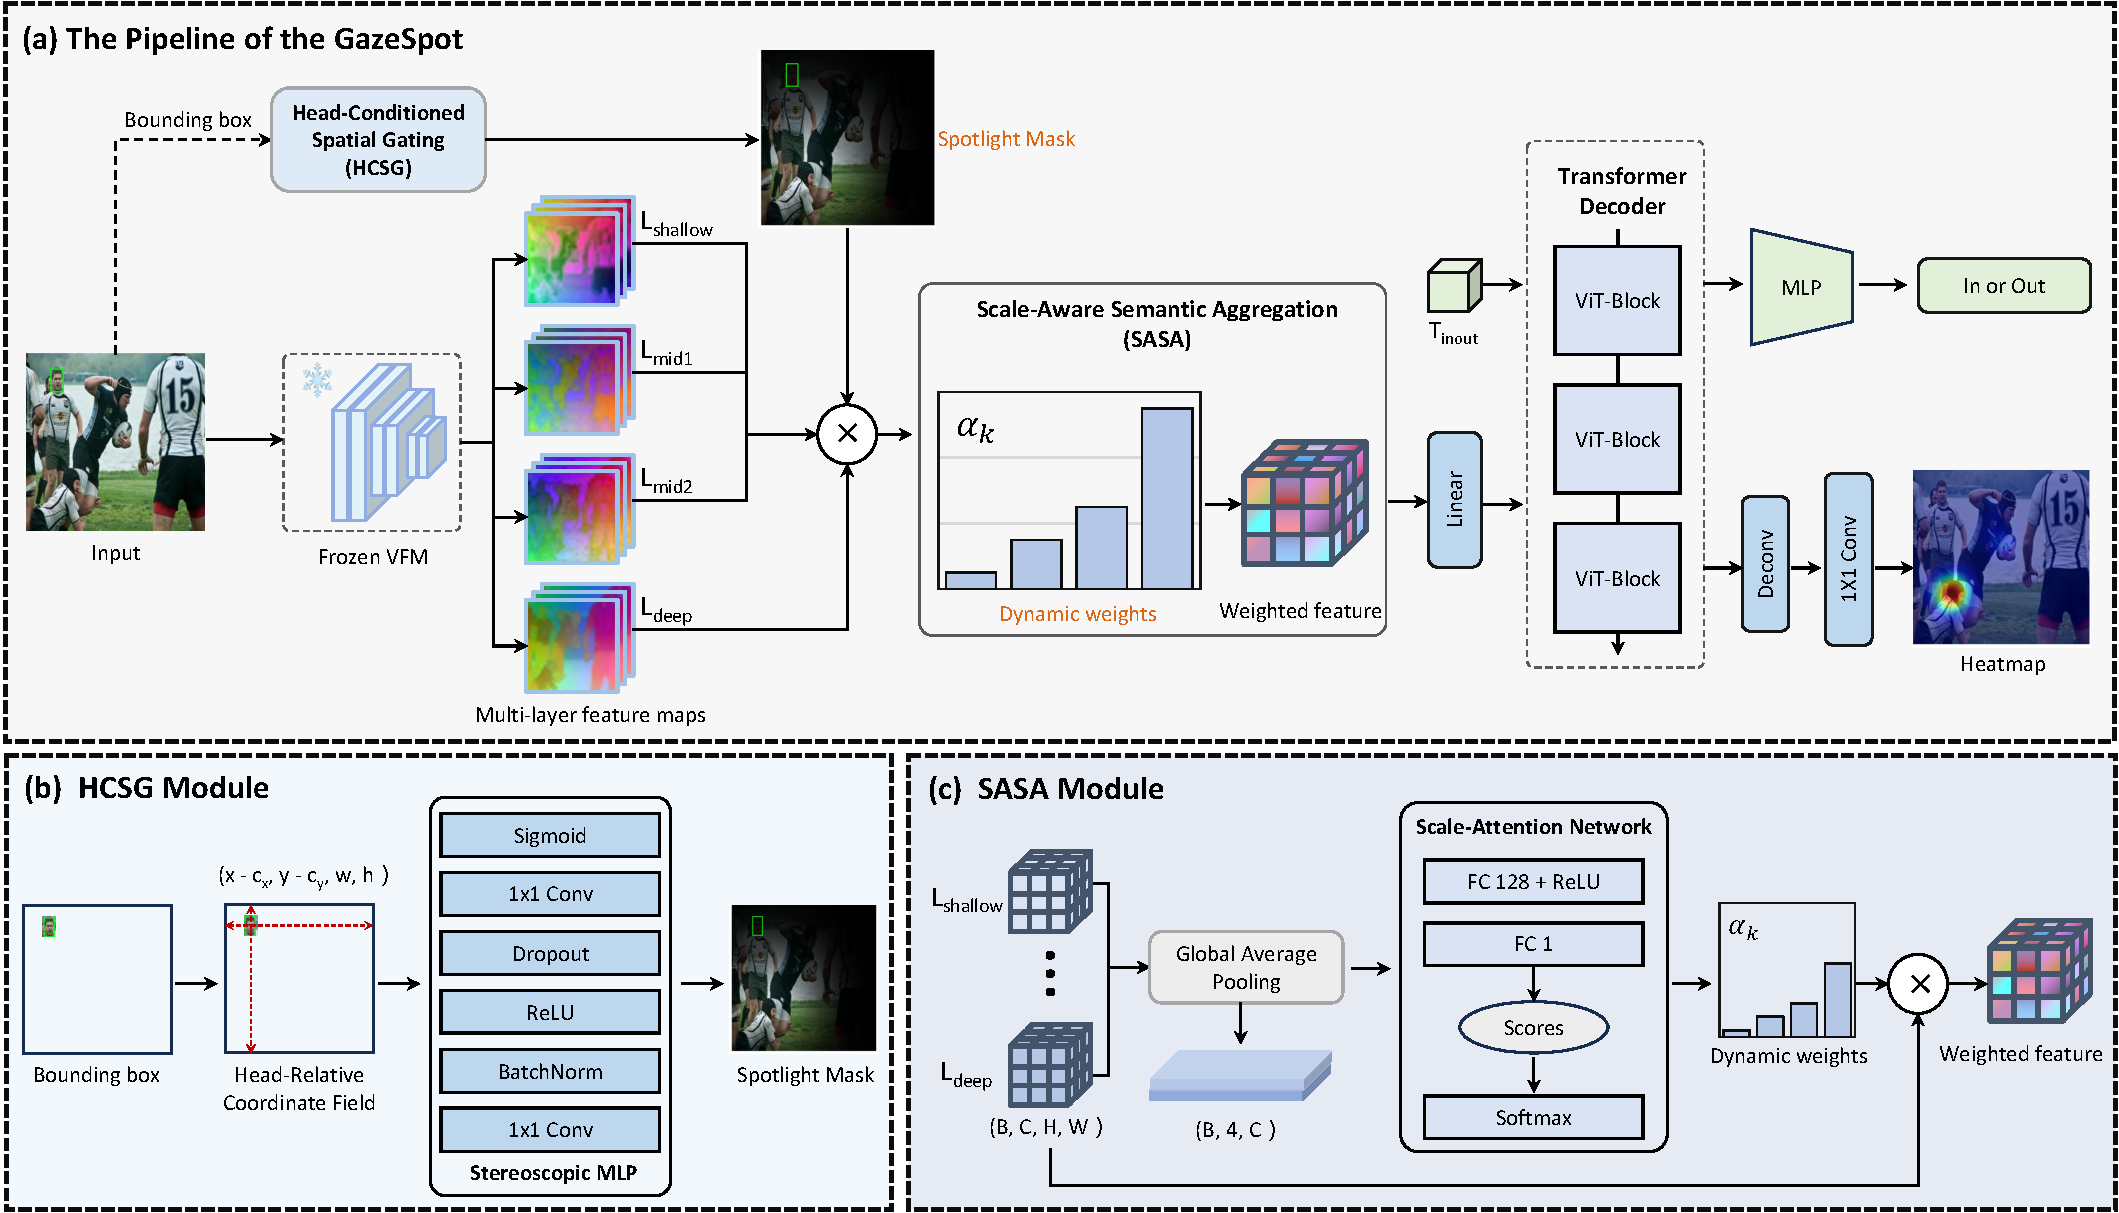
\includegraphics[width=0.94\textwidth]{img/icasspFig2.pdf}
  \caption{GazeSpot extracts four levels from a frozen VFM. HCSG applies a head-conditioned Spotlight Mask to each level, SASA fuses the gated features with image-dependent weights, and a lightweight decoder predicts the gaze heatmap and the in/out-of-frame score.}
  \label{fig:pipeline}
\end{figure*}

\begin{table*}[t]
  \centering
  \caption{Comparison with representative gaze target estimation methods on GazeFollow and VideoAttentionTarget. Competing results are taken from the corresponding papers, and ``Params'' denotes reported trainable parameters. Best and second-best values are bold and underlined.}
  \label{tab:sota}
  \setlength{\tabcolsep}{2.0pt}
  \renewcommand{\arraystretch}{1.00}
  \resizebox{\textwidth}{!}{%
  \begin{tabular}{llcccccccc}
    \toprule
    \multirow{2}{*}{Category} & \multirow{2}{*}{Method} & \multirow{2}{*}{Venue} & \multirow{2}{*}{Params} & \multicolumn{3}{c}{GazeFollow} & \multicolumn{3}{c}{VideoAttentionTarget}\\
    \cmidrule(lr){5-7}\cmidrule(lr){8-10}
    & & & & AUC $\uparrow$ & Avg $L_2$ $\downarrow$ & Min $L_2$ $\downarrow$ & AUC $\uparrow$ & $L_2$ $\downarrow$ & In/Out AP $\uparrow$\\
    \midrule
    \multirow{9}{*}{\shortstack[l]{Multi-branch /\\Multi-modal}}
    & Chong et al.~\cite{chong2018connecting} & ECCV 2018 & 51M & 0.896 & 0.187 & 0.112 & 0.833 & 0.171 & 0.712\\
    & Lian et al.~\cite{lian2018believe} & ACCV 2018 & 55M & 0.906 & 0.145 & 0.081 & 0.837 & 0.165 & --\\
    & Chong et al.~\cite{chong2020detecting} & CVPR 2020 & 61M & 0.921 & 0.137 & 0.077 & 0.860 & 0.134 & 0.853\\
    & Fang et al.~\cite{fang2021dual} & CVPR 2021 & 68M & 0.922 & 0.124 & 0.067 & 0.905 & 0.108 & 0.896\\
    & Bao et al.~\cite{bao2022escnet} & CVPR 2022 & 29M & 0.928 & 0.122 & -- & 0.885 & 0.120 & 0.869\\
    & Jin et al.~\cite{jin2022depth} & EAAI 2022 & 52M & 0.920 & 0.118 & 0.063 & 0.900 & 0.104 & 0.895\\
    & Miao et al.~\cite{miao2023patch} & WACV 2023 & 61M & 0.934 & 0.123 & 0.065 & 0.917 & 0.109 & \underline{0.908}\\
    & Tafasca et al.~\cite{tafasca2023childplay} & ICCV 2023 & 25M & 0.939 & 0.122 & 0.062 & 0.914 & 0.109 & 0.834\\
    & Sharingan~\cite{tafasca2024sharingan} & CVPR 2024 & 105M & 0.944 & 0.113 & 0.057 & -- & 0.107 & 0.891\\
    \midrule
    \multirow{4}{*}{\shortstack[l]{VFM-based /\\Single-branch}}
    & ViTGaze~\cite{song2024vitgaze} & VI 2024 & 22M & 0.949 & 0.105 & 0.047 & \underline{0.938} & \underline{0.102} & 0.905\\
    & GT360~\cite{dai2025gazetarget360} & IROS 2025 & 1.9M & 0.957 & 0.101 & -- & 0.934 & 0.103 & 0.887\\
    & Gaze-LLE (ViT-B)~\cite{ryan2025gaze} & CVPR 2025 & 2.8M & \underline{0.958} & 0.104 & 0.045 & 0.933 & 0.107 & 0.897\\
    & Gaze-LLE (ViT-L)~\cite{ryan2025gaze} & CVPR 2025 & 2.9M & \underline{0.958} & \underline{0.099} & \underline{0.041} & 0.937 & 0.103 & 0.903\\
    \midrule
    Ours & GazeSpot (ViT-L) & -- & 3.8M & \textbf{0.961} & \textbf{0.093} & \textbf{0.038} & \textbf{0.944} & \textbf{0.092} & \textbf{0.912}\\
    \bottomrule
  \end{tabular}}
\end{table*}


\section{Method}
\label{sec:method}

\subsection{Overview}
Given an image $I\in\mathbb R^{3\times H_I\times W_I}$ and a target head box $\mathbf b=[x_{\min},y_{\min},x_{\max},y_{\max}]$, GazeSpot predicts a heatmap $\hat{\mathbf M}\in[0,1]^{H_o\times W_o}$ and, when required, an in-frame probability $\hat p$. As shown in Fig.~\ref{fig:pipeline}, a frozen DINOv3 backbone supplies $K=4$ feature maps $\{\mathbf F_k\}_{k=1}^{K}$ sampled uniformly across its depth. Linear projections align their channel dimensions while retaining a common patch grid. The same scene features can therefore be reused for every annotated person; only the head box and the resulting Spotlight Mask change with the query.

The model has three stages. HCSG first converts the head box into a dense head-relative coordinate field and produces a Spotlight Mask that gates every feature level before aggregation. SASA then estimates image-dependent weights for the gated levels and projects their concatenation to a $D$-dimensional feature map. Finally, a lightweight Transformer jointly decodes the gaze heatmap and the in/out prediction. No object detector, segmentation model, depth estimator, or gaze-direction estimator is used during training or inference.

\subsection{Head-conditioned spatial gating}
Let $\mathbf c=(c_x,c_y)$, $w$, and $h$ denote the normalized center and size of the head box. At feature location $\mathbf p=(x,y)$, HCSG constructs a four-channel head-relative tensor
\begin{equation}
  \mathbf G(\mathbf p)=[x-c_x,\;y-c_y,\;w,\;h],
  \quad \mathbf G\in\mathbb R^{4\times H\times W}.
  \label{eq:geometry}
\end{equation}
A two-layer point-wise MLP, implemented with $1\times1$ convolutions, normalization, and ReLU, maps this field to a soft Spotlight Mask. The mask is broadcast along the channel dimension and applied to every selected level:
\begin{equation}
  \mathbf M_g=\sigma(\operatorname{MLP}(\mathbf G)), \qquad
  \mathbf F_k^g=\mathbf F_k\odot\mathbf M_g,\quad k=1,\ldots,K.
  \label{eq:gating}
\end{equation}
Using one Spotlight Mask across levels gives the feature hierarchy a consistent head-relative spatial bias, while leaving level selection to SASA. The mask does not encode a gaze vector or determine the final direction by itself; direction is inferred from the gated image evidence. It is learned end-to-end from the heatmap and in/out objectives, without mask supervision. We initialize the final MLP bias to $2$, keeping $\mathbf M_g$ close to one early in training and limiting disturbance to the pretrained features. Accordingly, the Spotlight Mask is a learned spatial gate, not a calibrated 3-D frustum or a hard field-of-view boundary.

\subsection{Adaptive multi-level fusion}
After spatial gating, SASA selects the feature granularity needed by the current scene. Global average pooling summarizes each gated feature as
\begin{equation}
  \mathbf v_k=\operatorname{GAP}(\mathbf F_k^g)
  =\frac{1}{HW}\sum_{i=1}^{H}\sum_{j=1}^{W}\mathbf F_k^g(i,j).
  \label{eq:gap}
\end{equation}
A shared two-layer scoring network $s(\cdot)$ evaluates these descriptors, and a Softmax across levels produces normalized weights
\begin{equation}
  \alpha_k=\frac{\exp s(\mathbf v_k)}{\sum_{j=1}^{K}\exp s(\mathbf v_j)},
  \qquad \sum_{k=1}^{K}\alpha_k=1.
  \label{eq:weights}
\end{equation}
The gated features are weighted, concatenated, and projected to the decoder dimension $D=256$:
\begin{equation}
  \mathbf X=\operatorname{Conv}_{1\times1}\!\left(
  \mathop{\Vert}_{k=1}^{K}\alpha_k\mathbf F_k^g\right).
  \label{eq:sasa}
\end{equation}
Here $\Vert$ denotes channel concatenation. Unlike fixed averaging, the weights vary with the image and target-conditioned features. Earlier levels can retain boundaries and local structure in crowded regions, while deeper levels provide the semantics needed to distinguish plausible targets. Concatenation preserves level-specific channels before the $1\times1$ projection mixes them.

\subsection{Gaze decoding}
We flatten $\mathbf X$ into a sequence $\mathbf S\in\mathbb R^{HW\times D}$. A learned 2-D positional embedding $\mathbf E_{\mathrm{pos}}$ preserves the patch layout. We also rasterize the query head box on the patch grid and map the binary head region to a learned embedding $\mathbf E_{\mathrm{head}}$. The decoder input is
\begin{equation}
  \mathbf S_{\mathrm{in}}=
  [\mathbf T_{\mathrm{in/out}};\,\mathbf S+\mathbf E_{\mathrm{pos}}+\mathbf E_{\mathrm{head}}],
  \label{eq:decoder_input}
\end{equation}
where $\mathbf T_{\mathrm{in/out}}\in\mathbb R^{1\times D}$ is a learned state token. Three Transformer blocks produce $[\hat{\mathbf T}_{\mathrm{in/out}};\hat{\mathbf S}]$. The state token is passed to an MLP for in-frame classification, while the patch tokens are reshaped and upsampled by a deconvolutional head:
\begin{equation}
  \hat p=\sigma(\operatorname{MLP}(\hat{\mathbf T}_{\mathrm{in/out}})),\qquad
  \hat{\mathbf M}=\sigma(\operatorname{Deconv}(\operatorname{Reshape}(\hat{\mathbf S}))).
  \label{eq:predictions}
\end{equation}

\subsection{Training objective}
The target heatmap $\mathbf M_{\mathrm{gt}}$ is formed by placing a Gaussian at the annotated fixation. Pixel-level binary cross-entropy supervises $\hat{\mathbf M}$, and a second binary cross-entropy term supervises $\hat p$ against the in-frame label $p_{\mathrm{gt}}$. The total loss is
\begin{equation}
  \mathcal L=\mathcal L_{\mathrm{heat}}+\lambda\mathcal L_{\mathrm{in/out}}.
  \label{eq:objective}
\end{equation}
For GazeFollow, which contains only in-frame annotations, $\lambda=0$. For VideoAttentionTarget (VAT), $\lambda=1$ and both branches are optimized jointly.

\section{Experiments}
\label{sec:experiments}

\subsection{Datasets and Evaluation Metrics}
We evaluate on GazeFollow~\cite{recasens2015they} and VideoAttentionTarget (VAT)~\cite{chong2020detecting}. AUC and Euclidean $L_2$ error measure localization. GazeFollow additionally reports minimum $L_2$ over its multiple annotations, while VAT reports average precision (AP) for in/out-of-frame prediction. For crowded-scene analysis, VAT test frames are divided by the number of annotated heads: fewer than three (7,945 frames), three (3,015), four (1,628), and more than four (539). We further use the real-image split of GOO~\cite{wang2022gatector} as an out-of-distribution (OOD) test for GazeFollow-trained checkpoints.

\subsection{Implementation Details}
Images are resized to $512\times512$ and heatmaps to $64\times64$. The DINOv3 backbone is frozen, the decoder dimension is 256, and training uses Adam with cosine learning-rate decay on one RTX 3090. Table~\ref{tab:sota} reports the complete HCSG+SASA model with a ViT-L backbone. The crowd, perturbation, GOO-real, and component-ablation analyses use ViT-B checkpoints to enable controlled comparisons with the reproduced last-layer baseline.

\subsection{Main results}
Table~\ref{tab:sota} compares GazeSpot-ViT-L with prior multi-branch and VFM-based methods. Relative to Gaze-LLE (ViT-L), GazeSpot improves GazeFollow AUC from 0.958 to 0.961, average $L_2$ from 0.099 to 0.093, and minimum $L_2$ from 0.041 to 0.038. On VAT, it improves AUC from 0.937 to 0.944, $L_2$ from 0.103 to 0.092, and in/out AP from 0.903 to 0.912, while retaining the single-branch frozen-backbone setting.

For a cross-dataset check, we directly evaluate the GazeFollow-trained ViT-B checkpoints on GOO-real without fine-tuning. We use the same split, preprocessing, checkpoint-selection rule, and evaluation script for the reproduced Gaze-LLE baseline and GazeSpot. As shown in Table~\ref{tab:goo}, GazeSpot improves AUC from 0.8583 to 0.8833 and reduces $L_2$ from 0.1997 to 0.1761. GOO-real has one target annotation per sample, so average and minimum $L_2$ are identical.

\begin{table}[t]
  \centering
  \caption{OOD evaluation on GOO-real using GazeFollow-trained checkpoints without fine-tuning.}
  \label{tab:goo}
  \renewcommand{\arraystretch}{1.05}
  \begin{tabular*}{\columnwidth}{@{\extracolsep{\fill}}lccc@{}}
    \toprule
    Method & AUC $\uparrow$ & Avg $L_2$ $\downarrow$ & Min $L_2$ $\downarrow$\\
    \midrule
    Reproduced Gaze-LLE & 0.8583 & 0.1997 & 0.1997\\
    GazeSpot & \textbf{0.8833} & \textbf{0.1761} & \textbf{0.1761}\\
    \bottomrule
  \end{tabular*}
\end{table}

\begin{table}[t]
  \centering
  \caption{Localization by crowd density on VAT. Relative $L_2$ reduction is computed against the last-layer baseline.}
  \label{tab:crowd}
  \renewcommand{\arraystretch}{1.05}
  \setlength{\tabcolsep}{3.2pt}
  \begin{tabular}{lcccccc}
    \toprule
    & & \multicolumn{2}{c}{Last-layer baseline} & \multicolumn{2}{c}{GazeSpot} & \multirow{2}{*}{\shortstack{Rel. $L_2$\\reduction}}\\
    \cmidrule(lr){3-4}\cmidrule(lr){5-6}
    Heads & Frames & AUC & $L_2$ & AUC & $L_2$ & \\
    \midrule
    $<3$ & 7,945 & 0.958 & 0.078 & 0.958 & \textbf{0.077} & 1.3\%\\
    $=3$ & 3,015 & 0.932 & 0.100 & \textbf{0.934} & \textbf{0.099} & 1.0\%\\
    $=4$ & 1,628 & 0.934 & 0.111 & \textbf{0.942} & \textbf{0.101} & 9.0\%\\
    $>4$ & 539 & 0.875 & 0.182 & \textbf{0.890} & \textbf{0.171} & 6.0\%\\
    \midrule
    $\geq4$ & 2,167 & 0.915 & 0.134 & \textbf{0.925} & \textbf{0.124} & \textbf{7.5\%}\\
    \bottomrule
  \end{tabular}
\end{table}

The density breakdown in Table~\ref{tab:crowd} shows little difference on sparse frames, but a larger gap as more people appear. The relative $L_2$ reduction reaches 9.0\% at exactly four heads and 6.0\% with more than four heads. On the combined subset with at least four heads, GazeSpot improves AUC from 0.915 to 0.925 and reduces $L_2$ by 7.5\%. Perturbing each head box by up to 20\% changes GazeSpot to 0.923/0.124, suggesting that the learned gate is not overly sensitive to moderate box noise.

\begin{figure}[t]
  \centering
  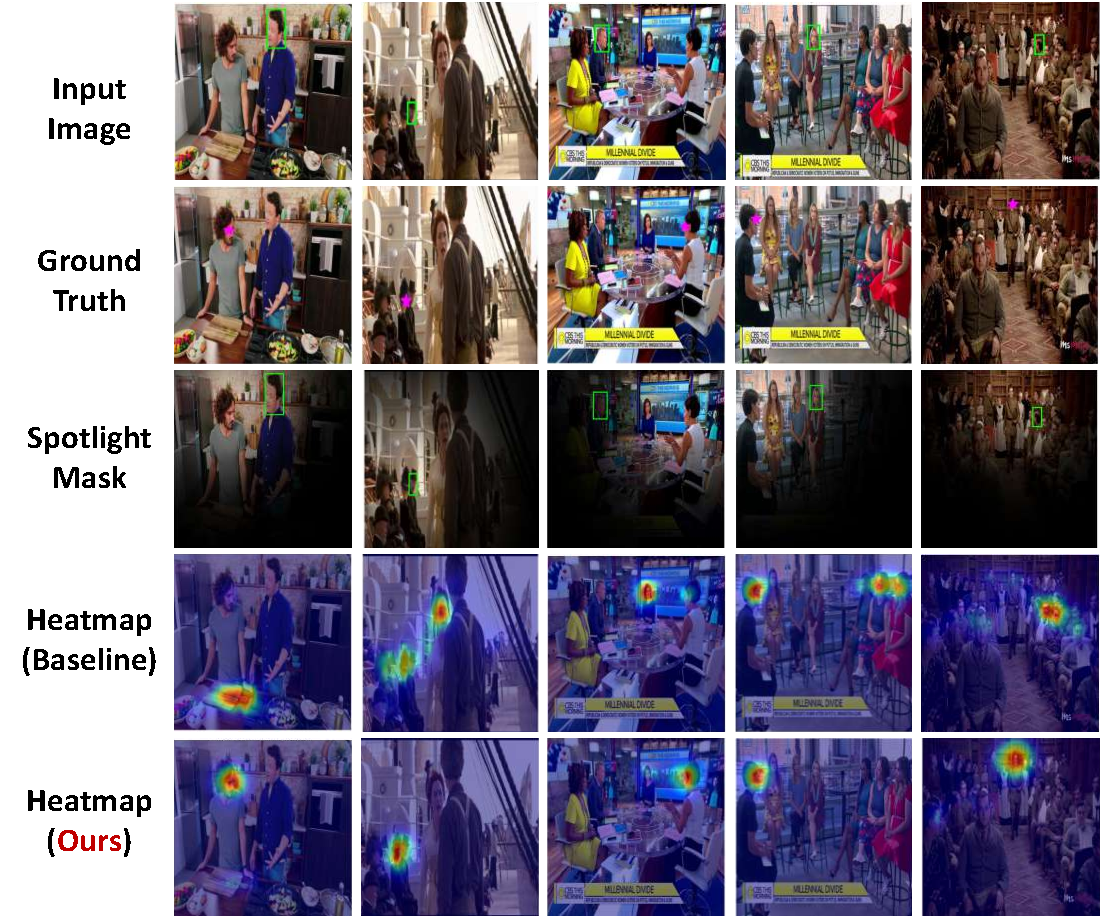
\includegraphics[width=0.85\columnwidth]{2026ACMMM/Figure/baseVSspot_compressed.pdf}
  \caption{Qualitative comparison on crowded VAT frames. From top to bottom: input and query head box, ground truth, Spotlight Mask, last-layer baseline heatmap, and GazeSpot heatmap.}
  \label{fig:crowd_visualization}
\end{figure}

\begin{table}[t]
  \centering
  \caption{Controlled ViT-B/16 analyses: (a) component ablation with DINOv3; (b) backbone comparison in $L_2$ error ($\downarrow$).}
  \label{tab:ablation}
  \label{tab:backbone}
  \renewcommand{\arraystretch}{1.05}
  \textit{(a) Component ablation}\\[1pt]
  \begin{tabular*}{\columnwidth}{@{\extracolsep{\fill}}ccc|cc|cc@{}}
    \toprule
    Multi-level & SASA & HCSG & \multicolumn{2}{c|}{GF} & \multicolumn{2}{c}{VAT}\\
    & & & AUC & $L_2$ & AUC & $L_2$\\
    \midrule
    & & & 0.955 & 0.107 & 0.933 & 0.106\\
    \checkmark & & & 0.957 & 0.103 & 0.937 & 0.103\\
    \checkmark & \checkmark & & 0.958 & 0.102 & 0.939 & 0.101\\
    \checkmark & \checkmark & \checkmark & \textbf{0.958} & \textbf{0.101} & \textbf{0.940} & \textbf{0.099}\\
    \bottomrule
  \end{tabular*}
  \\[4pt]
  \textit{(b) Backbone comparison}\\[1pt]
  \begin{tabular*}{\columnwidth}{@{\extracolsep{\fill}}lcccc@{}}
    \toprule
    & \multicolumn{2}{c}{Last-layer baseline} & \multicolumn{2}{c}{GazeSpot}\\
    \cmidrule(lr){2-3}\cmidrule(lr){4-5}
    Dataset & DINOv2 & DINOv3 & DINOv2 & DINOv3\\
    \midrule
    GazeFollow & \textbf{0.104} & 0.107 & 0.102 & \textbf{0.101}\\
    VAT & 0.107 & \textbf{0.106} & 0.104 & \textbf{0.099}\\
    Crowd ($\geq4$) & \textbf{0.133} & 0.139 & 0.132 & \textbf{0.124}\\
    \bottomrule
  \end{tabular*}
\end{table}

\subsection{Ablation Studies}
Table~\ref{tab:ablation}(a) separates the effect of multi-level features, adaptive fusion, and spatial gating. Raw multi-level fusion improves the last-layer baseline on both datasets. SASA provides a further reduction in $L_2$, and HCSG gives the best localization result without changing the backbone. For the ViT-B model, GazeSpot has 3.5M trainable and 89.2M total parameters, compared with 2.8M and 88.5M for the baseline. At $512\times512$, it requires 141.1 GFLOPs and 22.8 ms per image on an RTX 3090; the corresponding baseline uses 107.2 GFLOPs and 18.4 ms. The added robustness therefore comes with a measurable, but moderate, computation increase.

The ablation separates feature access from feature selection. Exposing all four levels accounts for most of the gain, while SASA and HCSG provide smaller, consistent improvements. Thus, the final layer is not always the best sole representation for localization; neither are shallow features uniformly preferable, since SASA retains the deep level and jointly selects contributions across the hierarchy.

\newpage
\textbf{Backbone analysis.} Table~\ref{tab:backbone}(b) shows that DINOv3 increases last-layer error on GazeFollow and crowded VAT frames, but slightly improves overall VAT. Combined with GazeSpot, it performs best on all three splits, supporting hierarchical features without attributing the difference to feature over-smoothing alone.

\section{Conclusion}
GazeSpot combines head-conditioned spatial gating with adaptive multi-level VFM fusion. Controlled ablations show that access to the feature hierarchy provides the main gain, while SASA and the Spotlight Mask offer complementary improvements. The advantage grows in crowded scenes and remains under moderate head-box perturbations. Zero-shot evaluation on GOO-real further shows that the improvement transfers beyond the training domain. Together, these results support head-conditioned multi-level decoding as a simple and effective alternative to pipelines that depend on external object masks or gaze-direction supervision.

\clearpage
\balance
\bibliographystyle{IEEEbib}
\bibliography{refs_icassp}

\end{document}
